\chapter{Immagini, tabelle, codice, liste}
In questo capitolo verranno spiegati tutti i comandi per inserire codice, tabelle di varie dimensioni, elenchi, immagini ecc.

\section{Inserimento di un'immagine}
Durante la produzione del testo può essere utile avere un'immagine o una serie di immagini.
\begin{figure}[H]
	\centering
	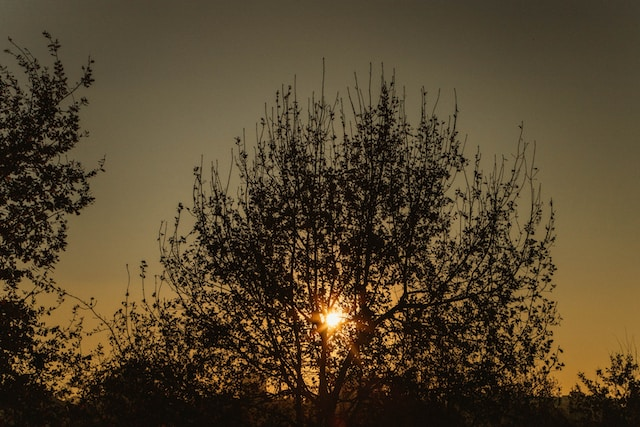
\includegraphics[scale=0.4]{image1} % Non è necessario specificare l'estensione. L'immagine viene pescata automaticamente dalla cartella 'img'
	\caption{Immagine singola centrata e scalata}
	\label{capitolo2:image1}
\end{figure}
È possibile fare riferimento alle immagini attraverso la sua label (figura \ref{capitolo2:image1}).\\   % Con questo \\ si va a capo
In altri casi è necessario avere più immagini affiancate.